\let\negmedspace\undefined
\let\negthickspace\undefined
\documentclass[journal]{IEEEtran}
\usepackage[a5paper, margin=10mm, onecolumn]{geometry}
%\usepackage{lmodern} % Ensure lmodern is loaded for pdflatex
\usepackage{tfrupee} % Include tfrupee package

\setlength{\headheight}{1cm} % Set the height of the header box
\setlength{\headsep}{0mm}     % Set the distance between the header box and the top of the text

\usepackage{gvv-book}
\usepackage{comment}
\usepackage{gvv}
\usepackage{cite}
\usepackage{amsmath,amssymb,amsfonts,amsthm}
\usepackage{algorithmic}
\usepackage{graphicx}
\usepackage{textcomp}
\usepackage{xcolor}
%\usepackage{txfonts}
\usepackage{listings}
\usepackage{enumitem}
\usepackage{mathtools}
\usepackage{gensymb}
\usepackage{comment}
\usepackage[breaklinks=true]{hyperref}
\usepackage{tkz-euclide} 
\usepackage{listings}
% \usepackage{gvv}                                        
\def\inputGnumericTable{}                                 
\usepackage[latin1]{inputenc}                                
\usepackage{color}                                            
\usepackage{array}                                            
\usepackage{longtable}                                       
\usepackage{calc}                                             
\usepackage{multirow}                                         
\usepackage{hhline}                                           
\usepackage{ifthen}                                           
\usepackage{lscape}
\usepackage{circuitikz}
\tikzstyle{block} = [rectangle, draw, fill=blue!20, 
    text width=4em, text centered, rounded corners, minimum height=3em]
\tikzstyle{sum} = [draw, fill=blue!10, circle, minimum size=1cm, node distance=1.5cm]
\tikzstyle{input} = [coordinate]
\tikzstyle{output} = [coordinate]


\begin{document}

\bibliographystyle{IEEEtran}
\vspace{3cm}

\title{12.27}
\author{EE25BTECH11013 - Bhargav}
\maketitle
    {\let\newpage\relax\maketitle}

\renewcommand{\thefigure}{\theenumi}
\renewcommand{\thetable}{\theenumi}
\setlength{\intextsep}{10pt} % Space between text and floats

\numberwithin{equation}{enumi}
\numberwithin{figure}{enumi}
\renewcommand{\thetable}{\theenumi}

\textbf{Question}: \\
1200 men and 500 women can build a bridge in 2 weeks. 900 men and 250 women will take 3 weeks to build the same bridge. How many men will be needed to build the bridge in one week? \\
\solution \\
Let one man complete work in X weeks and one woman complete work in Y weeks\\
In one week a man can complete $\frac{1}{X}$ work and woman can complete $\frac{1}{Y}$
\begin{align}
\frac{1200}{X} + \frac{500}{Y} = \frac{1}{2} \implies XY - 1000X - 2400Y = 0 \label{eq:1}
\end{align}
\begin{align}
\frac{900}{X} + \frac{250}{Y} = \frac{1}{3} \implies XY - 750X - 2700Y = 0 \label{eq:2}
\end{align}

Rotate the axis by $45\degree$ to remove the $XY$ term in the equations
\begin{align}
\vec{X} = \vec{Q}\vec{x} 
\end{align}
(where $\vec{Q}$ is the rotation matrix)
\begin{align}
\myvec{X \\ Y} = \myvec{\frac{1}{\sqrt{2}} & \frac{1}{\sqrt{2}} \\ \frac{1}{\sqrt{2}} & -\frac{1}{\sqrt{2}}}\myvec{x \\ y} \label{eq:3}
\end{align}
\begin{align}
\implies XY = \frac{x^2 - y^2}{2}
\end{align}
The conic equations become:
\begin{align}
x^2 - y^2 -3400\sqrt{2}x + 1400\sqrt{2}y = 0
\end{align}
\begin{align}
x^2 - y^2 - 3450\sqrt{2}x + 1950\sqrt{2}y = 0
\end{align}
These can be represented as general conic equations:
\begin{align}
\vec{x}^\top\vec{V}\vec{x} + 2\vec{u}^\top\vec{x} + f = 0
\end{align}\\ \\ \\ 
For the conics: $\vec{V} = \myvec{1 & 0 \\ 0 & -1}$, $\vec{u_1} = \myvec{-1700\sqrt{2} \\ 700\sqrt{2}}$, $\vec{u_2} = \myvec{-1725\sqrt{2} \\ 975\sqrt{2}}$, $f=0$

In homogeneous coordinates, using the form $\vec{x}^\top C \vec{x} = 0$, where $\vec{x} = \myvec{x & y & 1}^T$, the matrices for the conics are:\\
\begin{align}
\vec{C} = \myvec{\vec{V} & \vec{u^T} \\ \vec{u} & f}
\end{align}
\begin{align}
\implies \vec{C_1} = \myvec{1 & 0 & -1700\sqrt{2} \\ 0 & -1 & 700\sqrt{2} \\ -1700\sqrt{2} & 700\sqrt{2} & 0}
\end{align}
\begin{align}
\implies \vec{C_2} = \myvec{1 & 0 & -1725\sqrt{2} \\ 0 & -1 & 975\sqrt{2} \\ -1725\sqrt{2} & 975\sqrt{2} & 0}
\end{align}\\

The intersection point of both the conics lies on the conic formed by their individual linear combination $\vec{C(\mu)} = \vec{C_1} + \mu\vec{C_2}$. We must find the value of $\mu$ that makes the determinant of the conic's matrix as 0.
\begin{align}
\vec{C(\mu)} = \myvec{1+\mu & 0 & -1700\sqrt{2} -1725\sqrt{2}\mu \\ 0 & -\mu - 1 & 700\sqrt{2}+  975\sqrt{2}\mu \\ -1700\sqrt{2} -1725\sqrt{2}\mu & 700\sqrt{2}+ 975\sqrt{2}\mu & 0}
\end{align}
On solving $\det{\brak{\vec{C(\mu)}}}$ = 0, the simplest value of $\mu = -1$
\begin{align}
\brak{\vec{x}^\top\vec{V}\vec{x} + 2\vec{u_1}^\top\vec{x} + f} + \brak{-1}\brak{\vec{x}^\top\vec{V}\vec{x} + 2\vec{u_2}^\top\vec{x} + f} = 0
\end{align}
The chord of intersection of the 2 hyperbolas is:
\begin{align}
\vec{\brak{u_1^T - u_2^T}}\vec{x} = 0 \implies \myvec{1 & -11}\myvec{x \\ y} = 0
\end{align}

The point of intersection of the common chord and the first hyperbola can be found out by solving them
\begin{align}
\vec{x} = \vec{h} + k_i\vec{m}, \vec{h} = \myvec{0 \\ 0}, \vec{m} = \myvec{11 \\ 1}
\end{align}

\begin{align}
(\vec{h} + k_i \vec{m})^{\top} \vec{V} (\vec{h} + k_i \vec{m}) + 2\vec{u}^{\top} (\vec{h} + k_i \vec{m}) + f &= 0 \\
\implies k_i^{2} \vec{m}^{\top}\vec{V}\vec{m} + 2k_i \vec{m}^{\top} (\vec{V}\vec{h} + \vec{u}) + \vec{h}^{\top}\vec{V}\vec{h} + 2\vec{u}^{\top}\vec{h} + f &= 0 \\
\text{or, } k_i^{2} \vec{m}^{\top}\vec{V}\vec{m} + 2k_i \vec{m}^{\top} (\vec{V}\vec{h} + \vec{u}) + g(\vec{h}) &= 0
\end{align}

Solving the above quadratic gives the equation
\begin{align}
k_i = \frac{1}{\vec{m}^{\top}\vec{V}\vec{m}}
\brak{
    -\vec{m}^{\top} (\vec{V}\vec{h} + \vec{u})
    \;\pm\;
    \sqrt{ \sbrak{\vec{m}^{\top}(\vec{V}\vec{h} + \vec{u})}^2
    - g(\vec{h}) \, (\vec{m}^{\top}\vec{V}\vec{m}) }
    }
\end{align}
Solving we get:
\begin{align}
k_1 = 0, k_2 = 300\sqrt{2}
\end{align}

The point of intersection:
\begin{align}
\vec{x_1} = \myvec{0 \\ 0}, \vec{x_2} = \myvec{3300\sqrt{2} \\ 300\sqrt{2}}
\end{align}
The point $\vec{x_1} = \myvec{0 \\ 0}$ is not possible because it causes division by 0.\\

Substituting $\vec{x_2}$ in the rotation matrix equation:
\begin{align}
\vec{X} = \myvec{3600 \\ 3000}
\end{align}

A man can complete the work in 3600 weeks, a woman can complete the work in 3000 weeks
    \begin{figure}[H]
        \centering
        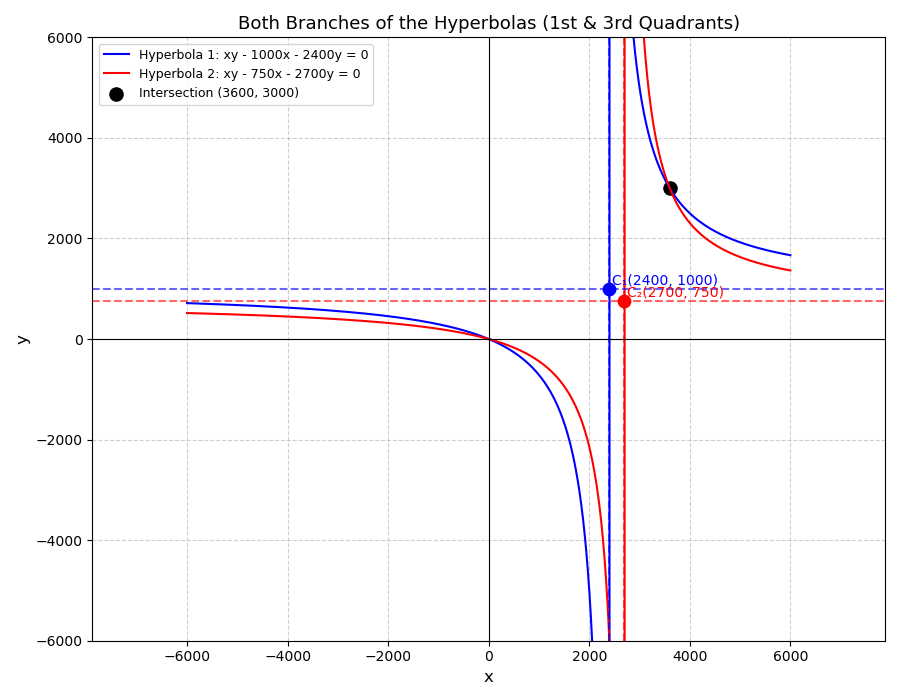
\includegraphics[height=0.5\textheight, keepaspectratio]{figs/Figure_1.png}
        \label{figure_1}
    \end{figure}

\end{document}
